%% LyX 2.4.0~beta5 created this file.  For more info, see https://www.lyx.org/.
%% Do not edit unless you really know what you are doing.
\documentclass[english]{foils}
\usepackage[T1]{fontenc}
\usepackage[latin9]{inputenc}
\pagestyle{foilheadings}
\setcounter{secnumdepth}{1}
\setcounter{tocdepth}{1}
\usepackage{xcolor}
\usepackage{pifont}
\usepackage{amsmath}
\usepackage{amsthm}
\usepackage{amssymb}
\usepackage{graphicx}

\makeatletter
%%%%%%%%%%%%%%%%%%%%%%%%%%%%%% Textclass specific LaTeX commands.
\theoremstyle{definition}
\newtheorem{defn}{\protect\definitionname}
\theoremstyle{remark}
\newtheorem{rem}{\protect\remarkname}
\newenvironment{lyxcode}
	{\par\begin{list}{}{
		\setlength{\rightmargin}{\leftmargin}
		\setlength{\listparindent}{0pt}% needed for AMS classes
		\raggedright
		\setlength{\itemsep}{0pt}
		\setlength{\parsep}{0pt}
		\normalfont\ttfamily}%
	 \item[]}
	{\end{list}}
\theoremstyle{remark}
\newtheorem*{rem*}{\protect\remarkname}

%%%%%%%%%%%%%%%%%%%%%%%%%%%%%% User specified LaTeX commands.
\usepackage{xcolor}
\renewcommand{\labelitemi}{$\textcolor{blue}{\bullet}$}
\renewcommand{\labelitemii}{$\textcolor{teal}{\Rightarrow}$}
\renewcommand{\labelitemiii}{$\textcolor{red}{\rightarrow}$}
\renewcommand{\labelitemiv}{$\textcolor{brown}{\circ}$}
% for French theorems, etc. since I'm using English to fix bullet pb.
\providecommand{\examplename}{Example}
\providecommand{\definitionname}{Definition}
\providecommand{\theoremnname}{Theorem}
\providecommand{\remarkname}{Remark}
\providecommand{\exercisename}{Exercise}
% DT book stuff
\newcommand{\argmin}{\operatornamewithlimits{argmin}} % for a "clean" argmin 
\newcommand{\T}{\mathrm{T}}  % transpose
\newcommand{\PP}{\mathrm{P}}  % probability
\newcommand{\dd}{\mathrm{d}} % integration dx
\newcommand{\ee}{\mathrm{e}} % exponential
\newcommand{\E}{\mathrm{E}} % expectation
%_%_%_%_%_%_%_%_
% for tikz drawings and cartoons
%_%_%_%_%_%_%_%_

\usepackage{tikz}

% for tikzit drawings
\usepackage{tikzit}
\input{flow.tikzstyles}


% for decision trees:
\tikzset{
	treenode/.style = {shape=rectangle, rounded corners,
		draw, align=center,
		top color=white, bottom color=blue!20},
	root/.style     = {treenode, font=\Large, bottom color=red!30},
	env0/.style     = {treenode, font=\large, bottom color=orange!30},
	env1/.style     = {treenode,  bottom color=green!30},
	env/.style      = {treenode, font=\ttfamily\normalsize},
    leaf/.style      = {treenode, font=\ttfamily\normalsize},
	dummy/.style    = {circle,draw}
}
\usetikzlibrary{positioning}

%_%_%_%_%_%_%_%_%_%_
% for algorithms and listings
%_%_%_%_%_%_%_%_%_%_

%\usepackage{algorithm_MA,algpseudocode}
%\usepackage{algorithmic}
\usepackage{algpseudocode}

%\floatstyle{ruled}
%\newfloat{algorithm}{tbp}
%\providecommand{\algorithmname}{Algorithm}
%\floatname{algorithm}{\protect\algorithmname}
%

% try and fix \Comment problem due to excessive defs in Chap. DA
\algrenewcommand{\algorithmiccomment}[1]{%
	\hfill$\triangleright$\ \textcolor{darkgray}{#1}}

\makeatother

\usepackage{babel}
\providecommand{\definitionname}{Definition}
\providecommand{\remarkname}{Remark}

\begin{document}

\MyLogo{SciML - AutoDiff}
\title{SciML - Automatic Differentiation}
\author{Mark Asch - IMU/VLP/CSU }
\date{2023}
\maketitle

\foilhead{Program}
\begin{enumerate}
\item Automatic differentiation for scientific machine learning:
\begin{enumerate}
\item \textcolor{red}{Differentiable programming with autograd and PyTorch.}
\item \textcolor{red}{Gradients, adjoints, backpropagation and inverse problems.}
\item Neural networks for scientific machine learning.
\item Physics-informed neural networks.
\item The use of automatic differentiation in scientific machine learning.
\item The challenges of applying automatic differentiation to scientific
applications.
\end{enumerate}
\end{enumerate}

\foilhead{Differentiable programming}
\begin{itemize}
\item Differential programming is a technique for \textcolor{magenta}{automatically
computing the derivatives} of functions. 
\item This can be done using a variety of techniques, including: 
\begin{itemize}
\item \textbf{Symbolic differentiation}: This involves using symbolic mathematics
to represent the function and its derivatives. This can be a powerful
technique, but it can be difficult to use for complex functions. 
\item \textbf{Numerical differentiation}: This involves using numerical
methods to approximate the derivatives of the function. This is a
simpler technique than symbolic differentiation, but it is less accurate. 
\item \textbf{\textcolor{magenta}{Automatic differentiation}}: This is a
technique that combines symbolic and numerical differentiation to
automatically compute the derivatives of functions. This is the most
powerful technique for differential programming, and it is the most
commonly used technique in scientific machine learning. 
\end{itemize}
\item The mathematical theory of differential programming is based on the
concept of \textcolor{magenta}{gradients}. 
\begin{itemize}
\item The gradient of a function is a vector that tells you how the function
changes as its input changes. In other words, the gradient of a function
tells you the direction of \textcolor{magenta}{steepest} ascent or
descent. 
\item The gradient of a function can be calculated using the \textcolor{magenta}{gradient
descent algorithm}. The gradient descent algorithm works by starting
at a point and then moving in the direction of the gradient until
it reaches a minimum or maximum. 
\item In ML, we use \textcolor{magenta}{stochastic gradient }optimization
methods
\end{itemize}
\item Differential programming can be used to solve a variety of problems
in scientific machine learning, including: 
\begin{itemize}
\item Calculating the \textcolor{magenta}{gradients of loss functions} for
machine learning models---this is important for training machine
learning models. 
\item Solving \textcolor{magenta}{differential equations}---this can be
used to model the behavior of physical systems. 
\item Performing \textcolor{magenta}{optimization}---this can be used to
find the optimal solution to a problem.
\item Solving \textbf{\textcolor{magenta}{inverse and data assimilation
problems}}---this is none other than a special case of optimization.
\end{itemize}
\end{itemize}

\foilhead{$\;$}

\vfill{}

\begin{center}
{\Large\textbf{\textcolor{blue}{OPTIMIZATION}}}{\Large\par}
\par\end{center}

\vfill{}


\foilhead{Recall: Optimization}
\begin{itemize}
\item Optimization routines typically use \textcolor{magenta}{local information}
about a function to iteratively approach a \textcolor{magenta}{local
minimum.}
\end{itemize}
\begin{center}
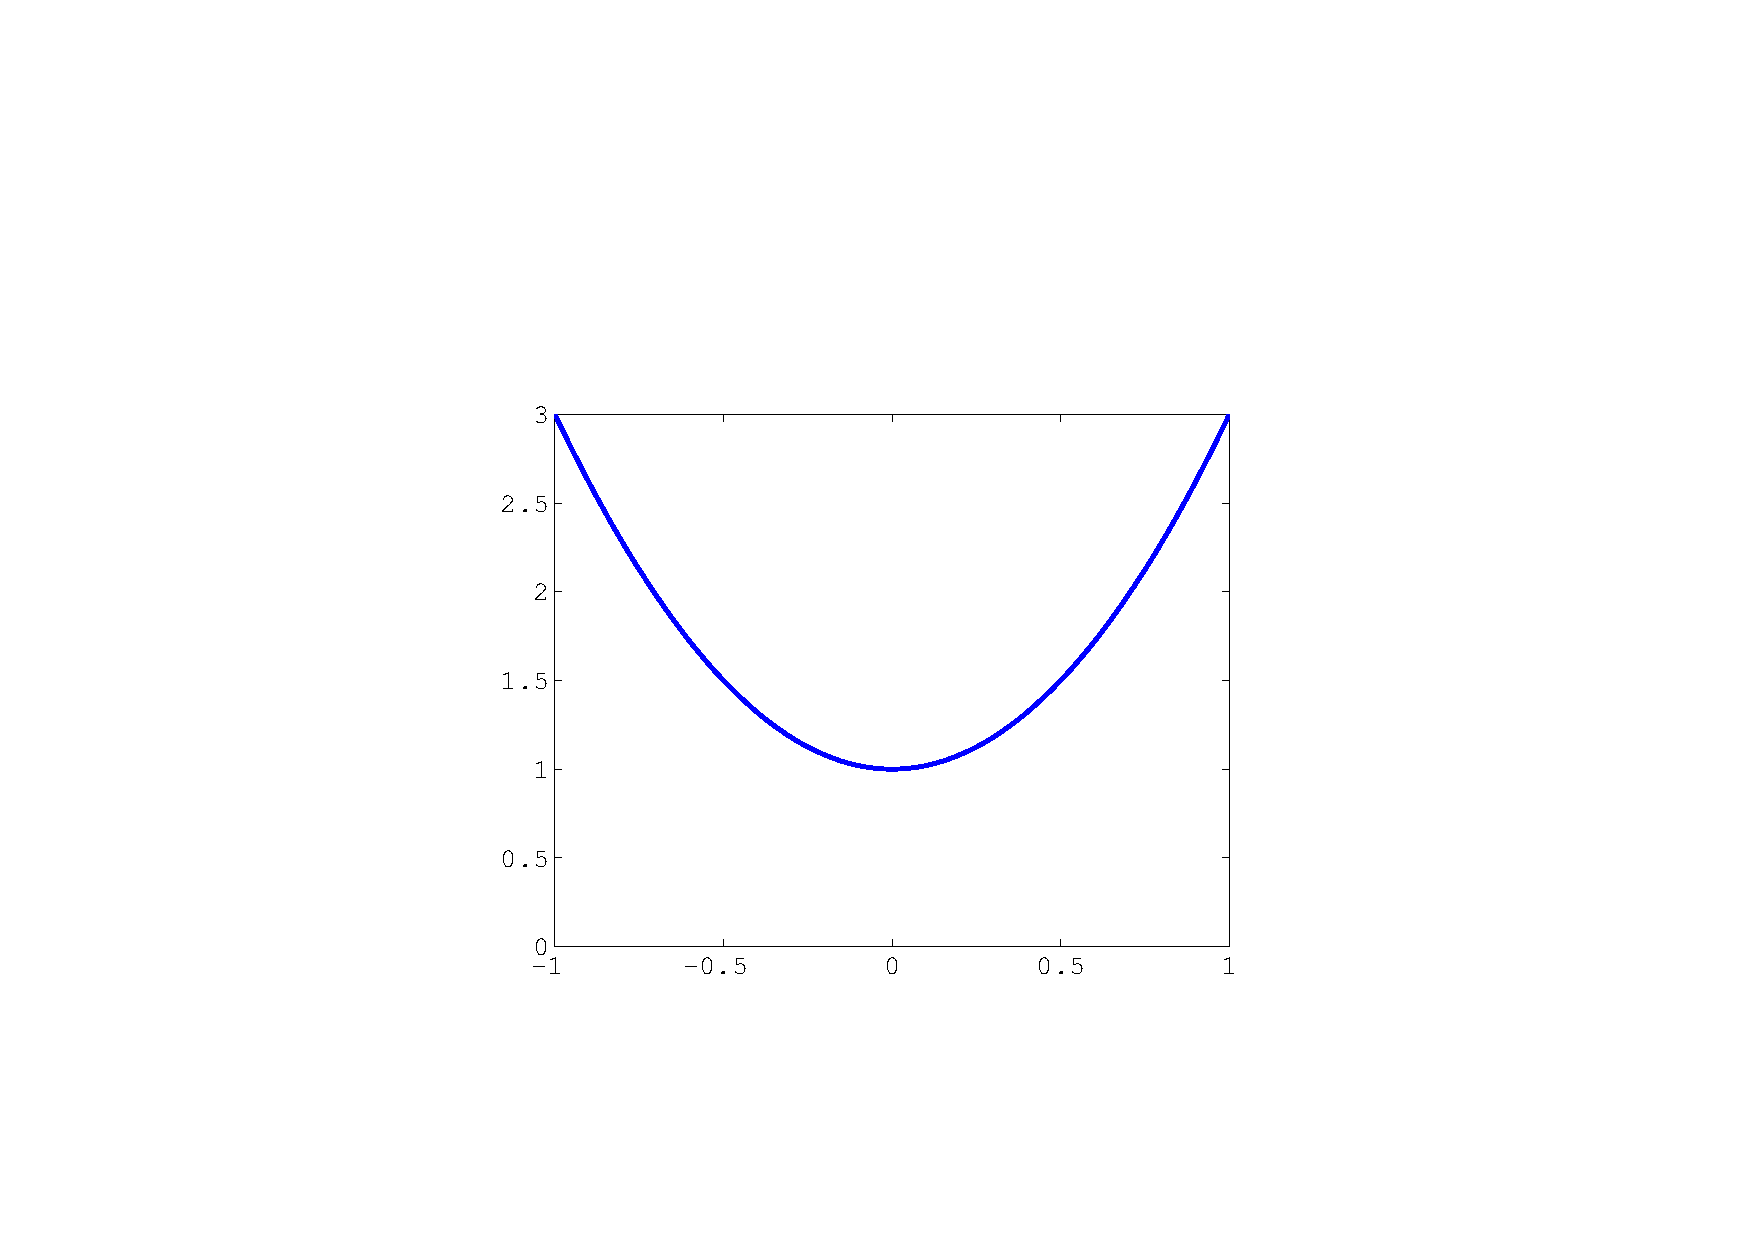
\includegraphics{graphics/am205_lec16-NL-opt-cnvx}
\par\end{center}
\begin{itemize}
\item In this (rare) case, where we have a \textcolor{magenta}{convex} function,
we easily find a global minimum.
\end{itemize}
\begin{center}
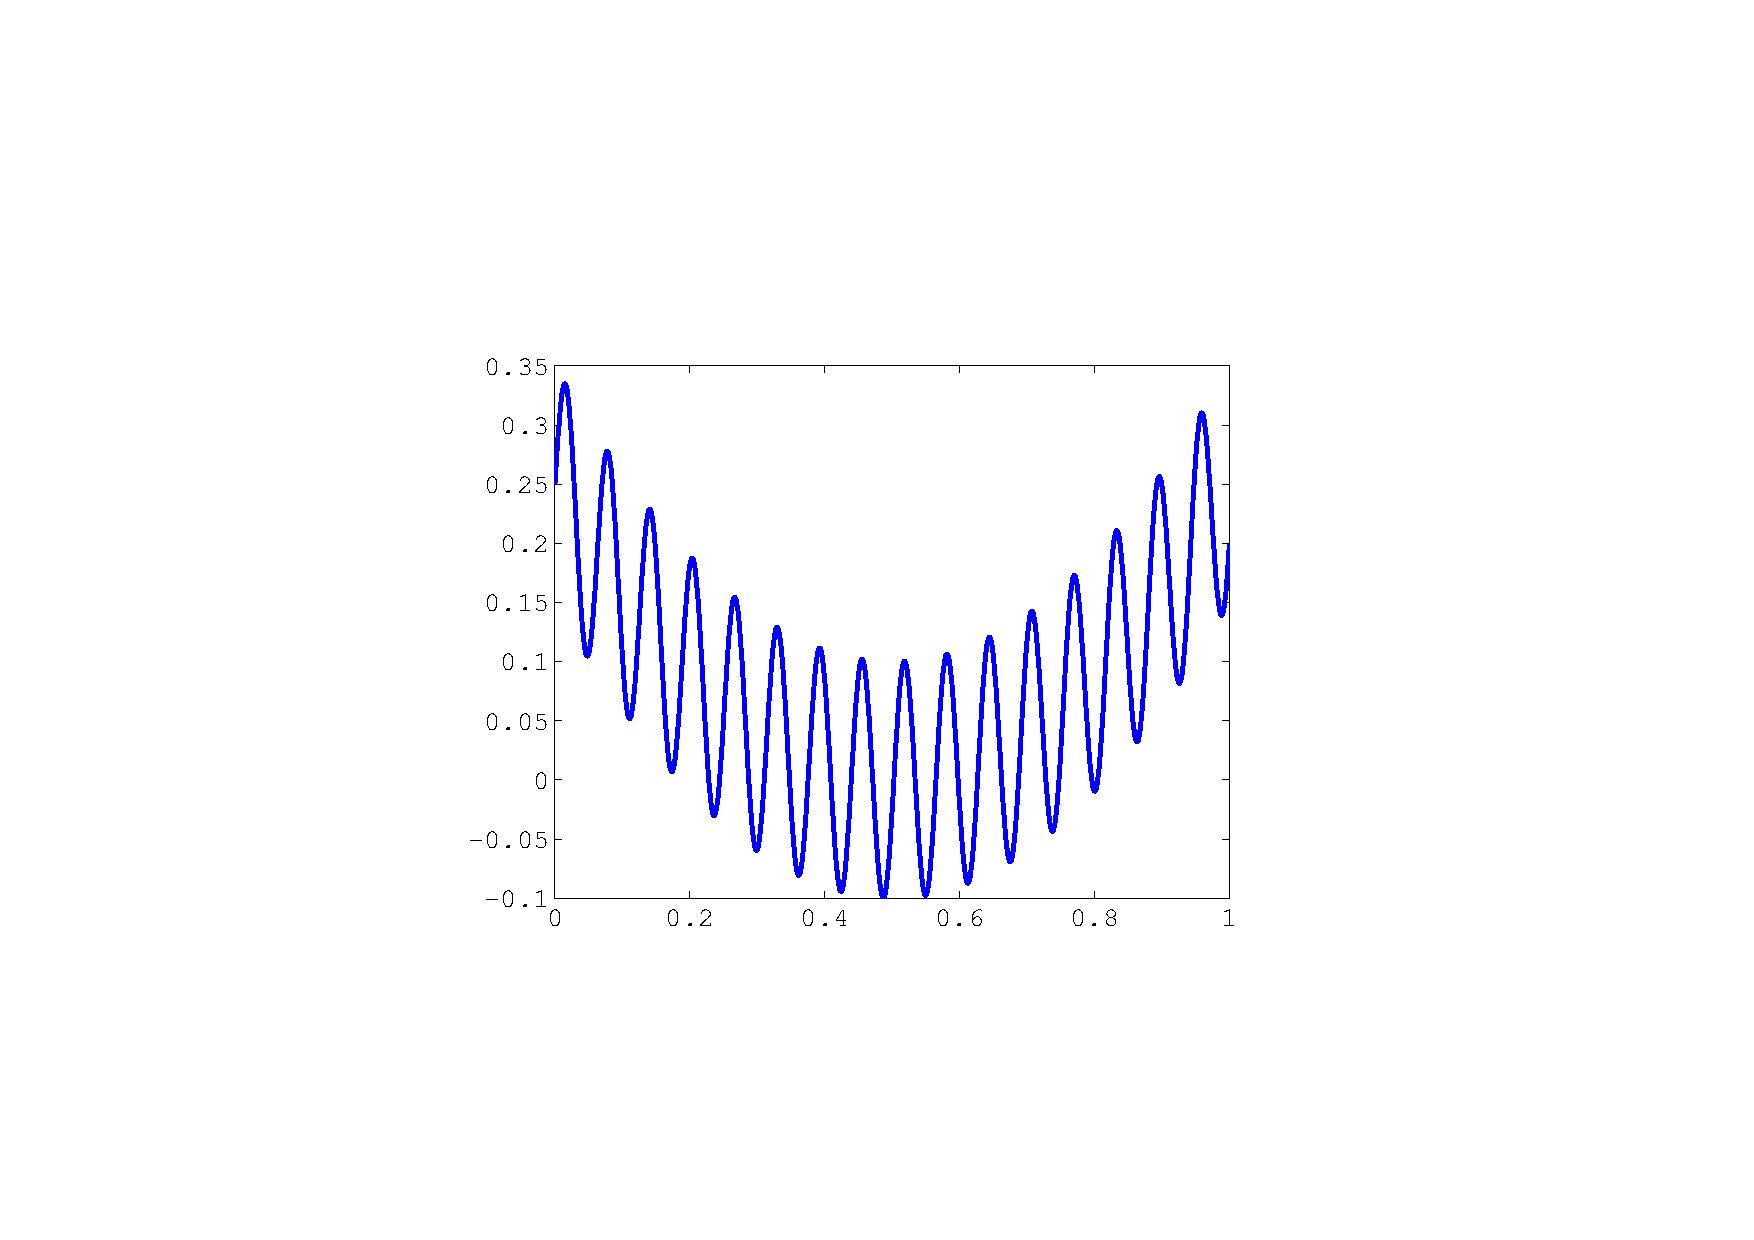
\includegraphics{graphics/am205_lec16-NL-opt-multi}
\par\end{center}
\begin{itemize}
\item But in general, global optimization can be very difficult
\begin{itemize}
\item \textcolor{red}{we usually get stuck in local minima!}
\end{itemize}
\end{itemize}
\begin{center}
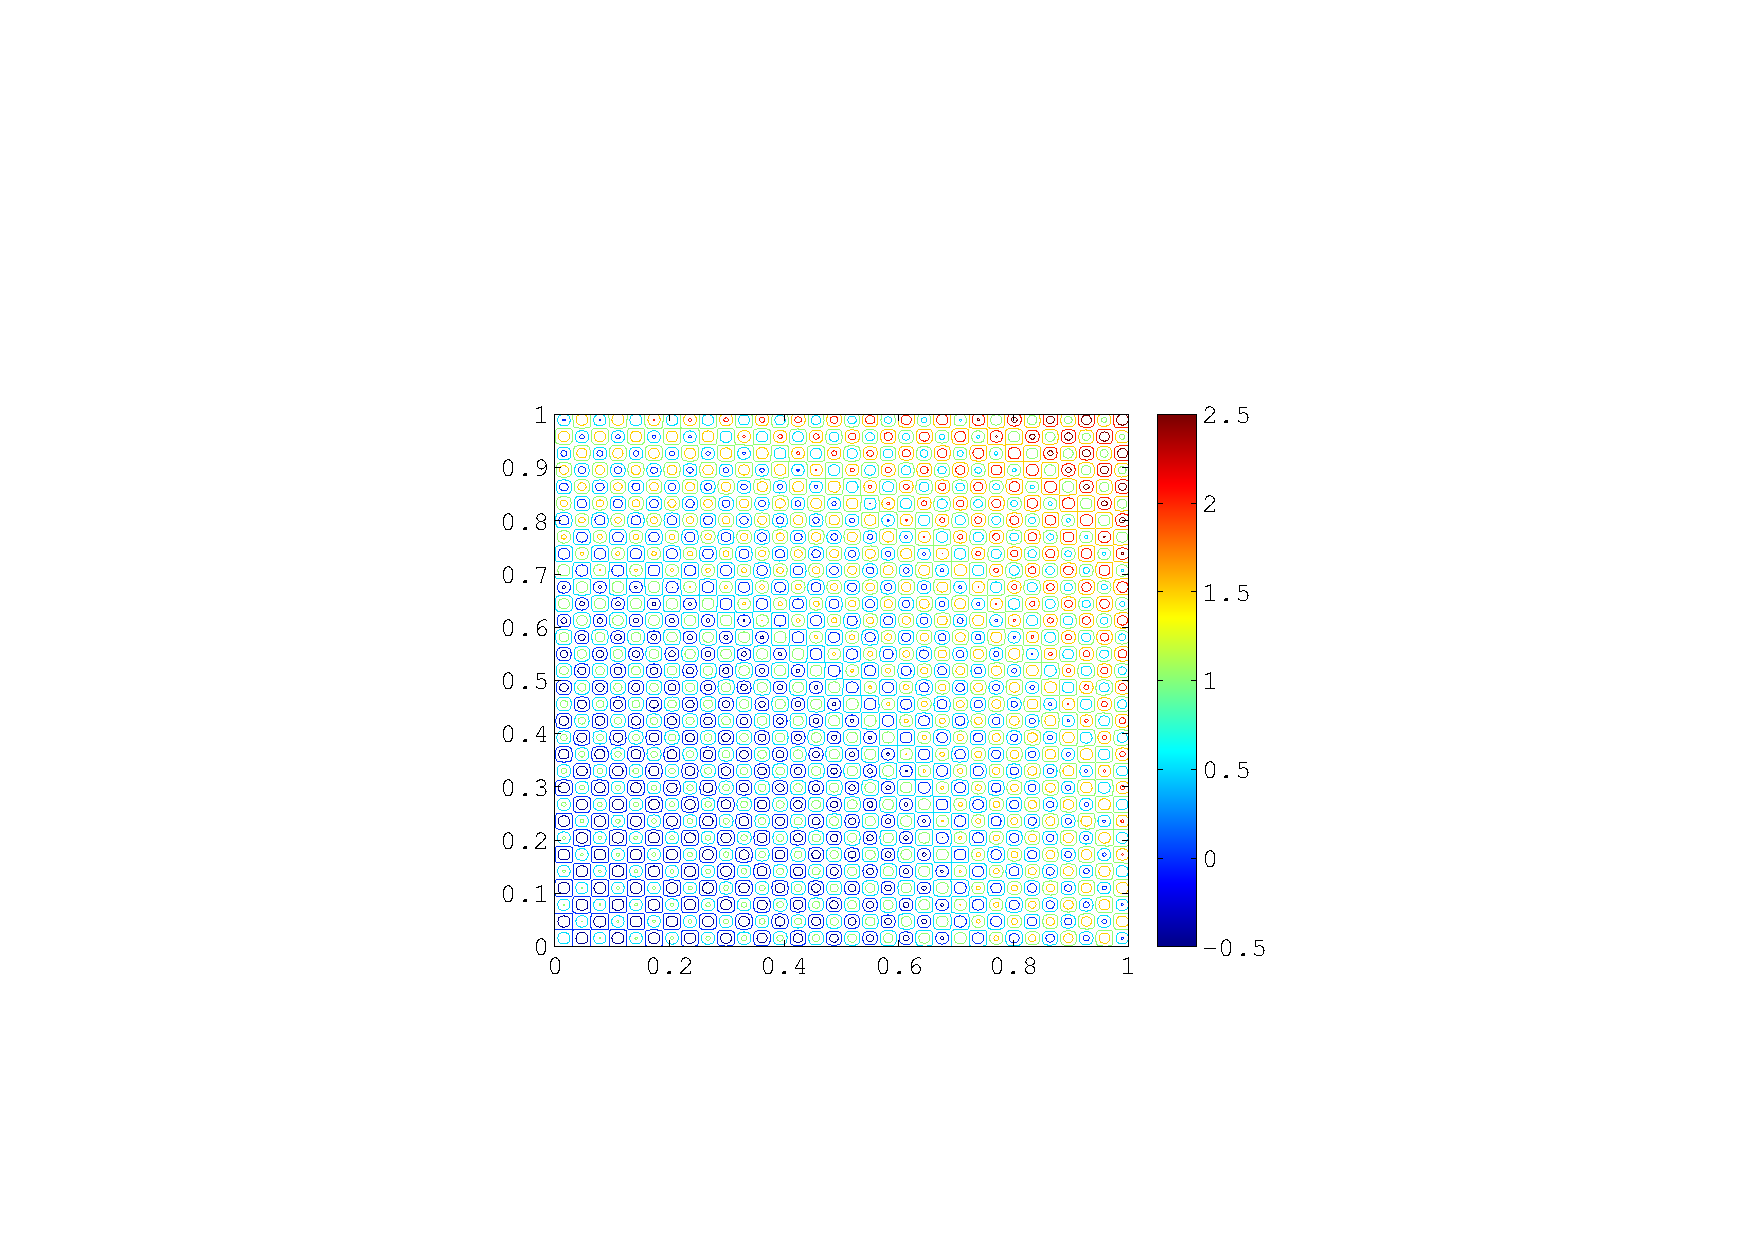
\includegraphics{graphics/am205_lec16-NL-opt-2D}
\par\end{center}
\begin{itemize}
\item Things get MUCH harder in\textcolor{magenta}{{} higher spatial dimensions}...
\begin{itemize}
\item and much worse when there is some \textcolor{magenta}{noise} in the
system.
\end{itemize}
\end{itemize}

\foilhead{$\;$}

\vfill{}

\begin{center}
{\Large\textbf{\textcolor{blue}{DIFFERENTIAL PROGRAMMING}}}{\Large\par}
\par\end{center}

\vfill{}


\foilhead{Recall: Differentiable Programming}

There are 3 ways to compute derivatives of functions:
\begin{enumerate}
\item \textcolor{magenta}{Symbolic} differentiation.
\item \textcolor{magenta}{Numerical} differentiation.
\item \textcolor{magenta}{Automatic} differentiation.
\end{enumerate}
\begin{itemize}
\item See \texttt{\textcolor{blue}{04\_diff\_prog}} for simple examples
of each of these.
\item See \texttt{\textcolor{blue}{04\_diff\_Autograd}} for use of \texttt{\textcolor{blue}{Autograd}}
\item See \textcolor{blue}{PyTorch} tutorials for much more extensive use
of AD in numerous optimization, ML and SciML cases.
\end{itemize}

\foilhead{Symbolic Differentiation}
\begin{itemize}
\item Computes exact, \textcolor{magenta}{analytical} derivatives, in the
form of a mathematical expression.
\begin{itemize}
\item There is no approximation error.
\item Operates recursively by applying simple rules to symbols.
\end{itemize}
\end{itemize}
\begin{dinglist}{56}
\item There may be no analytical expression for gradients of some functions.
\item Can lead to redundant and overly complex expressions.
\end{dinglist}
\begin{itemize}
\item Based on the \texttt{\textcolor{blue}{sympy}} package of Python.
\item Other software: Mathematica, Maple, Sage, etc.
\end{itemize}

\foilhead{Numerical Differentiation}
\begin{defn}
If $f$ is a differentiable function, then
\[
f'(x)=\lim_{h\rightarrow0}\frac{f(x+h)-f(x)}{h}
\]
\end{defn}
\begin{itemize}
\item Using Taylor expansions, and the definition of the derivative, we
can obtain finite-difference, \textcolor{magenta}{numerical approximations
}to the derivatives of $f,$ such as
\[
f'(x)=\frac{f(x+h)-f(x)}{h}+\mathcal{O}(h),
\]
\[
f'(x)=\frac{f(x+h)-f(x-h)}{2h}+\mathcal{O}(h^{2})
\]
{\small{} }{\small\par}
\begin{itemize}
\item conceptually simple and very easy to code
\item curse of dimensionality: to compute gradients of $f\colon\mathbb{R}^{m}\rightarrow\mathbb{R},$
requires at least $\mathcal{O}(m)$ function evaluations
\item big numerical errors due to truncation and roundoff.
\end{itemize}
\end{itemize}

\foilhead{$\;$}

\vfill{}

\begin{center}
{\Large\textbf{\textcolor{blue}{AUTOMATIC DIFFERENTIATION}}}{\Large\par}
\par\end{center}

\vfill{}


\foilhead{Automatic Differentiation}
\begin{itemize}
\item Automatic differentiation is an \textcolor{magenta}{umbrella term}
for a variety of techniques for efficiently computing accurate derivatives
of more or less general programs. 
\begin{itemize}
\item It is employed by all major neural network frameworks, where a single
reverse-mode AD backpass (also known as \textcolor{magenta}{``backpropagation''})
can compute a full gradient.
\item Numerical differentiation would either require many forward passes
or symbolic differentiation that is simply untenable due to expression
explosion. 
\item The survey paper \cite{Baydin2018} provides an excellent review of
all the methods and tools available.
\end{itemize}
\item Many algorithms in machine learning, computer vision, physical simulation,
and other fields require the calculation of gradients and other derivatives. 
\begin{itemize}
\item \textcolor{magenta}{Manual} derivation of gradients can be both time-consuming
and error-prone. 
\item \textcolor{magenta}{Automatic} differentiation comprises a set of
techniques to calculate the derivative of a numerical computation
expressed as a \textcolor{magenta}{computer code. }
\item These techniques of AD, commonly used for \textcolor{magenta}{data
assimilation} in atmospheric sciences and optimal design in computational
fluid dynamics, have more recently also been adopted by machine learning
researchers. 
\item The \textcolor{magenta}{backpropagation} algorithm, used for optimally
computing the weights of a neural network, is just a special case
of general AD. 
\item AD can be found in all the major software libraries for ML/DL, such
as TensorFlow, \textcolor{magenta}{PyTorch}, JaX. 
\item It is also found in the most recent implementations of MCMC that are
based on Hamiltonian Monte Carlo (HMC), such as Stan, PyMC3, Pyro
and others---see lecture on \textcolor{magenta}{Probabilistic Programming}.
\end{itemize}
\item Practitioners across many fields have built a wide set of \textcolor{magenta}{automatic
differentiation tools}, using different programming languages, computational
primitives, and intermediate compiler representations. 
\begin{itemize}
\item Each of these choices comes with positive and negative trade-offs,
in terms of their usability, flexibility, and performance in specific
domains. 
\item Nevertheless, the availability of such tools should not be neglected,
since the potential gain from their use is very large. 
\item Moreover, the fact that they are already built-in to a large number
of ML methods, makes their use quite straightforward.
\end{itemize}
\item AD can be readily and extensively used and is thus applicable to many
industrial and practical \textcolor{magenta}{Digital Twin} contexts
\cite{Asch2022}.
\end{itemize}

\foilhead{AD for SciML}
\begin{itemize}
\item Recent progress in machine learning (ML) technology has been spectacular.
\item At the heart of these advances is the ability to obtain high-quality
solutions to\textcolor{magenta}{{} non-convex optimization problems}
for functions with billions---or even hundreds of billions---of
parameters.
\item Incredible \textcolor{magenta}{opportunity} for progress in classical
applied mathematics problems. 
\begin{itemize}
\item In particular, the increased proficiency for systematically handling
large, non-convex optimization scenarios may help solve some classical
problems that have long been a challenge. 
\item We now have the chance to make substantial headway on questions that
have not yet been formulated or studied because we lacked the \textcolor{magenta}{tools}
to solve them. 
\item To be clear, we do not wish to oversell the state of the art, however: 
\begin{itemize}
\item Algorithms that identify the\textcolor{magenta}{{} global optimum} for
non-convex optimization problems do not yet exist. 
\item The ML community has instead developed efficient, open source software
tools that find \textcolor{magenta}{candidate} solutions.
\item They have created \textcolor{magenta}{benchmarks} to measure solution
quality.
\item They have cultivated a culture of \textcolor{magenta}{competition}
against these benchmarks.
\end{itemize}
\end{itemize}
\end{itemize}

\foilhead{Automatic Differentiation---backprop, autograd, etc.}
\begin{itemize}
\item \textcolor{magenta}{Backprop} is a special case of autodiff.
\item \textcolor{magenta}{Autograd} is a particular autodiff package.
\item In practice, we will pricipally use \textcolor{magenta}{PyTorch}'s
autodiff functions.
\end{itemize}
\begin{rem}
Autodiff is \textcolor{magenta}{NOT} finite differences, nor symbolic
differentiation. Finite differences are too \textcolor{magenta}{expensive}
(one forward pass for each discrete point). They induce huge \textcolor{magenta}{numerical
errors} (truncation/approximation and roundoff) and are very unstable
in the presence of noise.
\end{rem}
~
\begin{rem}
Autodiff is both \textcolor{magenta}{efficient}---linear in the cost
of computing the value---and numerically \textcolor{magenta}{stable}. 
\end{rem}
~
\begin{rem}
The goal of autodiff is not a formula, but a \textcolor{magenta}{procedure}
for computing derivatives.
\end{rem}

\foilhead{Tools for AD}
\begin{itemize}
\item New opportunities that exist because of the widespread, open-source
deployment of effective \textcolor{magenta}{software tools for automatic
differentiation}. 
\item While the \textcolor{magenta}{mathematical framework} for automatic
differentiation was established long ago---dating back at least to
the evolution of adjoint-based optimization in optimal control\cite{Asch2016,Asch2022}---ML
researchers have recently designed efficient software frameworks that
natively run on \textcolor{magenta}{hardware accelerators} (GPUs). 
\item These frameworks have served as a core technology for the ML revolution
over the last decade and inspired \textcolor{magenta}{high-quality
software} libraries such as 
\begin{itemize}
\item JAX, 
\item \textcolor{magenta}{PyTorch},
\item TensorFlow. 
\end{itemize}
\item The technology\textquoteright s key feature is: \textbf{the computational
cost of computing derivatives of a target loss function is independent
of the number of parameters;}
\begin{itemize}
\item this trait makes it possible for users to implement \textcolor{magenta}{gradient-based
optimization} algorithms for functions with staggering numbers of
parameters.
\end{itemize}
\end{itemize}

\foilhead{AD Sayings}
\begin{quote}
\textcolor{orange}{``Gradient descent can write code better than you,
I'm sorry.'' }

\textcolor{orange}{``Yes, you should understand backprop.'' }

\textcolor{orange}{``I've been using PyTorch a few months now and
I've never felt better. I have more energy. My skin is clearer. My
eye sight has improved.''}
\end{quote}
\begin{itemize}
\item Andrej Karpathy {[}\textasciitilde 2017{]} (Tesla AI, OpenAI)
\end{itemize}

\foilhead{$\;$}

\vfill{}

\begin{center}
{\Large\textbf{\textcolor{blue}{BACKPROPAGATION}}}{\Large\par}
\par\end{center}

\vfill{}


\foilhead{Backpropagation: optimization problem}
\begin{itemize}
\item We want to solve a (nonlinear, non-convex) \textcolor{magenta}{optimization
problem} (in very high dimensions), either 
\begin{itemize}
\item for a \textcolor{magenta}{dynamic system},
\[
\frac{\mathrm{d}\mathbf{x}}{\mathrm{d}t}=f(\mathbf{x};\mathbf{\theta}),
\]
where $\mathbf{x}\in\mathbb{R}^{n}$ and $\mathbf{\theta}\in\mathbb{R}^{p}$
with $n,p\gg1.$
\item or for a \textcolor{magenta}{machine learning} model
\[
\mathbf{y}=f(\mathbf{x};\mathbf{w}),
\]
where $\mathbf{x}\in\mathbb{R}^{n}$ and $\mathbf{w}\in\mathbb{R}^{p}$
with $n,p\gg1.$
\end{itemize}
\item To find the \textcolor{magenta}{minimum/optimum}, we want to minimize
an appropriate \textcolor{magenta}{cost/loss function}
\[
J(\mathbf{x},\mathbf{\theta}),\quad\mathcal{L}(\mathbf{w},\mathbf{\theta})
\]
 usually some\textcolor{magenta}{{} error norm}, and then (usually)
compute its average
\item The best/fastest way to solve this optimization problem, is to use
\textcolor{magenta}{gradients} and gradient-based methods.
\end{itemize}

\foilhead{Backpropagation: definition}
\begin{itemize}
\item Backpropagation is an algorithm for computing \textcolor{magenta}{gradients}.
\item Backpropagation is an instance of \textcolor{magenta}{reverse mode
automatic differentiation}
\begin{itemize}
\item very broadly applicable to machine learning, \textcolor{magenta}{data
assimilation} and inverse problems in general
\item it is \textquotedblleft just\textquotedblright{} a clever and efficient
use of the \textcolor{magenta}{Chain Rule }for derivatives
\end{itemize}
\end{itemize}

\foilhead{Backpropagation: theory}
\begin{itemize}
\item We can prove \textcolor{magenta}{mathematically} the following equivalences:
\begin{itemize}
\item Backpropagation\\
\textcolor{white}{equivale}$\Updownarrow$
\item Reverse-mode automatic differentiation\\
\textcolor{white}{equivale}$\Updownarrow$
\item Discrete adjoint-state method
\end{itemize}
\item Recall: the adjoint-state method is the theoretical basis for \textcolor{magenta}{Data
Assimilation}, as well as many other inverse problems---see Basic
Course, Lecture on Adjoint Methods (\textcolor{blue}{11\_DA\_adj.pdf}).
\end{itemize}

\foilhead{Recap: Gradient Descent }
\begin{itemize}
\item Recall: gradient descent moves opposite the gradient, hence in the
direction of \textcolor{magenta}{steepest descent}
\end{itemize}
\begin{center}
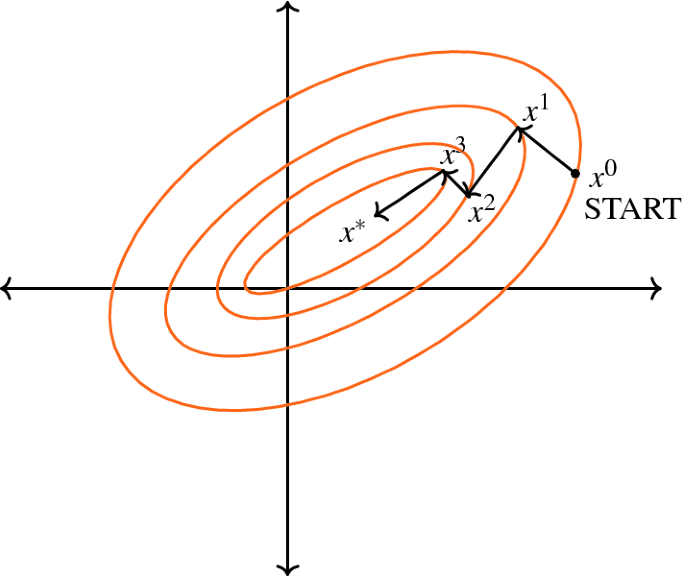
\includegraphics[scale=0.5]{graphics/sd}
\par\end{center}
\begin{itemize}
\item What is the optimization parameter space?
\begin{itemize}
\item one coordinate for each weight or bias of the network, in all the
layers, for a multilayer neural net
\item parameter values at all discrete points, for a (discretized) differential
equation
\begin{itemize}
\item very \textcolor{magenta}{high dimensional}
\item very hard to visualize
\end{itemize}
\end{itemize}
\item we want to compute the cost/loss function gradient, which is usually
the average over the training samples of the \textcolor{magenta}{loss
gradient},
\[
\nabla_{w}\mathcal{L}=\frac{\partial\mathcal{L}}{\partial w},\quad\nabla_{\theta}\mathcal{L}=\frac{\partial\mathcal{L}}{\partial\theta},
\]
 or, in general
\[
\nabla_{z}\mathcal{L}=\frac{\partial\mathcal{L}}{\partial z},
\]
 where $z=w$ or $z=\theta,$ etc.
\end{itemize}

\foilhead{Recap: Chain Rule}
\begin{itemize}
\item Recall: if $f(x)$ and $x(t)$ are \textcolor{magenta}{univariate}
(differentiable) functions, then
\[
\frac{\mathrm{d}}{\mathrm{d}t}f(x(t))=\frac{\mathrm{d}f}{\mathrm{d}x}\frac{\mathrm{d}x}{\mathrm{d}t}
\]
\item and this can be easily generalized to the \textcolor{magenta}{multivariate}
case, such as
\[
\frac{\mathrm{d}}{\mathrm{d}t}f(x(t),y(t))=\frac{\mathrm{d}f}{\mathrm{d}x}\frac{\mathrm{d}x}{\mathrm{d}t}+\frac{\mathrm{d}f}{\mathrm{d}y}\frac{\mathrm{d}y}{\mathrm{d}t}
\]
\end{itemize}

\foilhead{Chain Rule - a simple example}
\begin{itemize}
\item Consider
\[
f(x,y,z)=(x+y)z
\]
\item Decompose $f$ into \textcolor{magenta}{simple differentiable elements}
\[
q(x,y)=x+y,
\]
 then
\[
f=qz
\]
\item \textbf{Note}: each element has an \textcolor{magenta}{analytical}
(exact/known) derivative---eg. sums, products, sines, cosines, min,
max, exp, log, etc.
\item Now we can compute the gradient of $f$ with respect to its three
variables, using the \textcolor{magenta}{chain rule}
\begin{itemize}
\item we begin with 
\[
\frac{\partial f}{\partial q}=z,\quad\frac{\partial f}{\partial z}=q
\]
 and
\[
\frac{\partial q}{\partial x}=1,\quad\frac{\partial q}{\partial y}=1
\]
\item then the \textcolor{magenta}{chain rule} gives the terms of the \textcolor{magenta}{gradient},
\begin{align*}
\frac{\partial f}{\partial x} & =\frac{\partial f}{\partial q}\frac{\partial q}{\partial x}=z\cdot1\\
\frac{\partial f}{\partial y} & =\frac{\partial f}{\partial q}\frac{\partial q}{\partial y}=z\cdot1\\
\frac{\partial f}{\partial z} & =q
\end{align*}
\end{itemize}
\end{itemize}

\foilhead[-0.5in]{Here is a Python code snippet}
\begin{lyxcode}
\textcolor{gray}{\#~set~some~inputs~}

\textcolor{teal}{x~=~-2;~y~=~5;~z~=~-4}

\textcolor{gray}{\#~perform~the~forward~pass}\textcolor{teal}{{}~}

\textcolor{teal}{q~=~x~+~y~}\textcolor{gray}{\#~q~becomes~3}\textcolor{teal}{{}~}

\textcolor{teal}{f~=~q~{*}~z~}\textcolor{gray}{\#~f~becomes~-12}

\textcolor{gray}{\#~perform~the~backward~pass~(backpropagation)}

\textcolor{gray}{\#~in~reverse~order:~}

\textcolor{gray}{\#~first~backprop~through~f~=~q~{*}~z~}

\textcolor{teal}{dfdz~=~q~}\textcolor{gray}{\#~df/dz~=~q,~so~gradient~on~z~becomes~3~}

\textcolor{teal}{dfdq~=~z~}\textcolor{gray}{\#~df/dq~=~z,~so~gradient~on~q~becomes~-4~}

\textcolor{teal}{dqdx~=~1.0~}

\textcolor{teal}{dqdy~=~1.0~}

\textcolor{gray}{\#~now~backprop~through~q~=~x~+~y}\textcolor{teal}{{}~}

\textcolor{teal}{dfdx~=~dfdq~{*}~dqdx~~}\textcolor{gray}{\#~The~{*}~here~is~the~chain~rule!~}

\textcolor{teal}{dfdy~=~dfdq~{*}~dqdy~}~
\end{lyxcode}
\begin{itemize}
\item We obtain the \textcolor{magenta}{gradient} in the variables \texttt{\textcolor{teal}{{[}dfdx,
dfdy, dfdz{]}}} that give us the \textcolor{magenta}{sensitivity}
of the function \texttt{\textcolor{teal}{f}} to the variables \texttt{\textcolor{teal}{x,
y}} and \texttt{\textcolor{teal}{z}}.
\end{itemize}

\foilhead{Computational Graphs}
\begin{itemize}
\item It's all done with \textcolor{magenta}{graphs}... DAGs, in fact
\item The above computation can be visualized with a circuit diagram:
\end{itemize}
\begin{center}
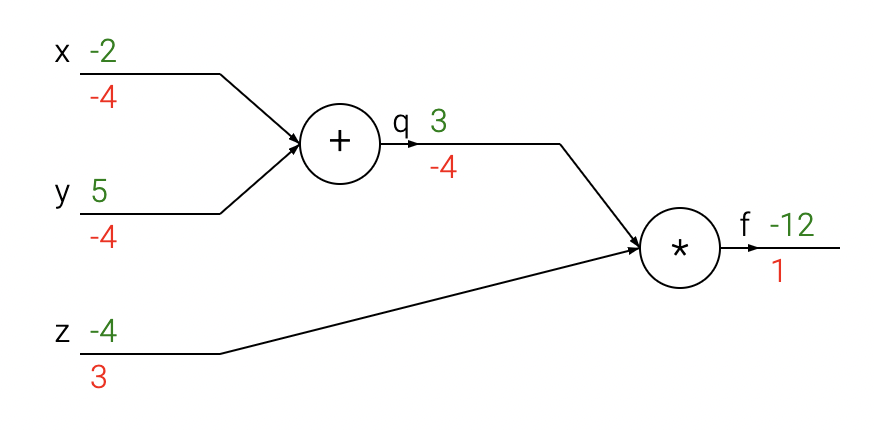
\includegraphics{graphics/comp_graph_simple}
\par\end{center}
\begin{itemize}
\item the\textcolor{green}{{} forward pass}, computes values from inputs to
outputs
\item the \textcolor{red}{backward pass} then performs backpropagation,
starting at the end and recursively applying the chain rule to compute
the gradients all the way to the inputs of the circuit. 
\begin{itemize}
\item The gradients can be thought of as \textcolor{magenta}{flowing backwards}
through the circuit.
\end{itemize}
\end{itemize}

\foilhead{Forward vs Reverse Mode}
\begin{itemize}
\item \textcolor{magenta}{Forward} mode is used for
\begin{itemize}
\item solving nonlinear equations
\item sensitivity analysis
\item uncertainty propagation/quantification
\[
f(x+\Delta x)\approx f(x)+f'(x)\Delta x
\]
\end{itemize}
\item \textcolor{magenta}{Reverse} mode is used for
\begin{itemize}
\item machine/deep learning
\item optimization
\end{itemize}
\end{itemize}

\foilhead{Backprop - ML example}
\begin{itemize}
\item For a univariate, logistic least-squares problem, we have:
\begin{itemize}
\item \textcolor{magenta}{linear model}/function of $x$: $z=wx+b$
\item \textcolor{magenta}{nonlinear activation}: $y=\sigma(x)$
\item \textcolor{magenta}{quadratic loss}: $\mathcal{L}=(1/2)(y-t)^{2},$
where $t$ is the target/observed value
\end{itemize}
\item \textbf{Objective}: find the values of the parameters/weights, $w$
and $b,$ that \textcolor{magenta}{minimize} the loss $\mathcal{L}$
\begin{itemize}
\item to do this, we will use the \textcolor{magenta}{gradient} of $\mathcal{L}$
with respect to the parameters/weights, $w$ and $b,$
\[
\nabla_{w}\mathcal{L}=\frac{\partial\mathcal{L}}{\partial w},\quad\nabla_{b}\mathcal{L}=\frac{\partial\mathcal{L}}{\partial b}
\]
\end{itemize}
\end{itemize}

\foilhead[-0.5in]{Calculus Approach}
\begin{itemize}
\item \textcolor{magenta}{Calculus} approach:
\end{itemize}
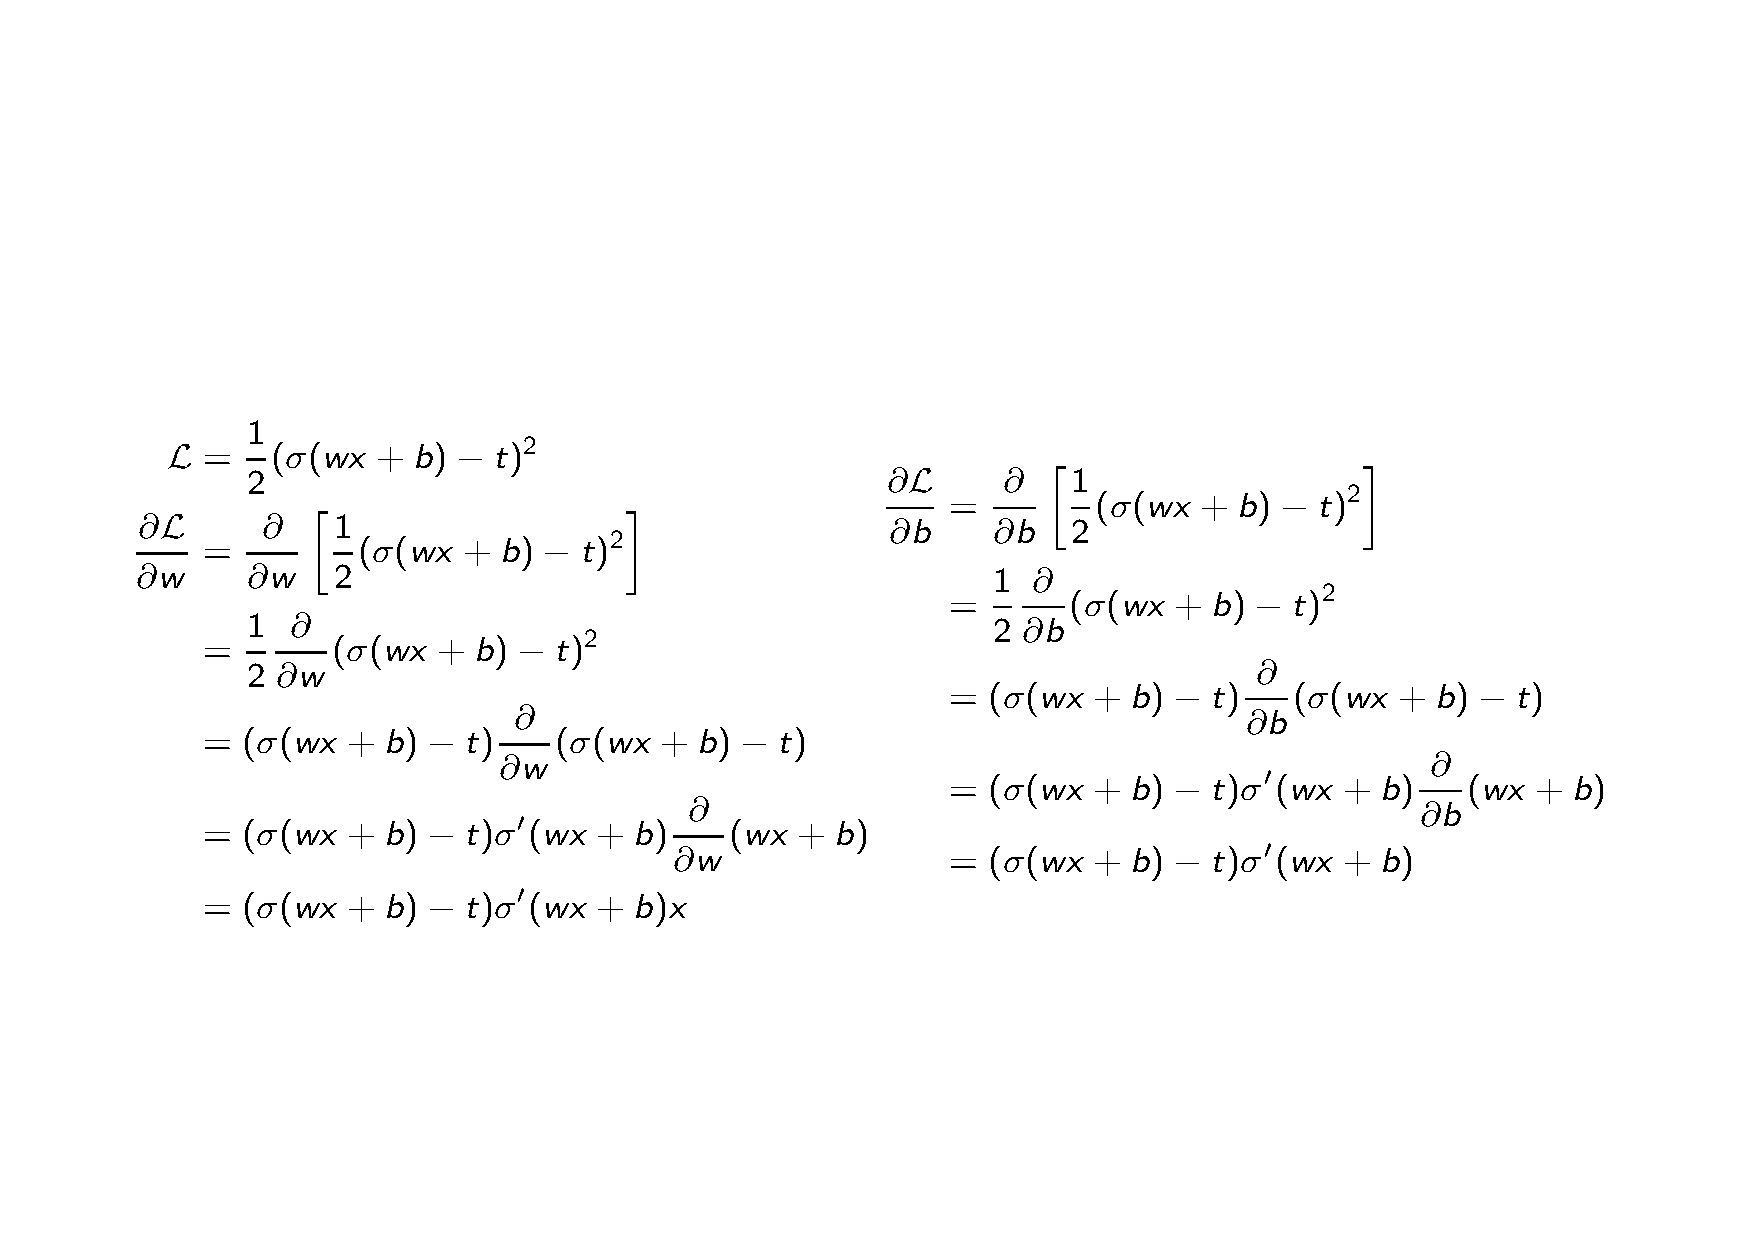
\includegraphics[width=1.15\textwidth]{graphics/univariate_chain}
\begin{itemize}
\item \textcolor{magenta}{It's a mess}... too many computations, too complex
to program!
\item \textcolor{magenta}{Structured} approach:
\begin{align*}
 & \mathrm{compute\ loss} &  & \mathrm{compute\ derivatives}\\
 & \mathrm{{\color{blue}forwards}} &  & \mathrm{{\color{red}backwards}}\\
z & =wx+b & \frac{\partial\mathcal{L}}{\partial y} & =y-t\\
y & =\sigma(z) & \frac{\partial\mathcal{L}}{\partial z} & =\frac{\partial\mathcal{L}}{\partial y}\frac{\partial y}{\partial z}=\frac{\partial\mathcal{L}}{\partial y}\sigma'(z)\\
\mathcal{L} & =\frac{1}{2}(y-t)^{2} & \frac{\partial\mathcal{L}}{\partial w} & =\frac{\partial\mathcal{L}}{\partial z}\frac{\partial z}{\partial w}=\frac{\partial\mathcal{L}}{\partial z}x\\
 &  & \frac{\partial\mathcal{L}}{\partial b} & =\frac{\partial\mathcal{L}}{\partial z}\frac{\partial z}{\partial b}=\frac{\partial\mathcal{L}}{\partial z}\cdot1
\end{align*}

\begin{itemize}
\item can easily be written as a \textcolor{magenta}{computational graph
}with
\begin{itemize}
\item nodes = inputs and computed quantities
\item edges = nodes computed directly as functions of other nodes
\end{itemize}
\end{itemize}
\end{itemize}
\begin{center}
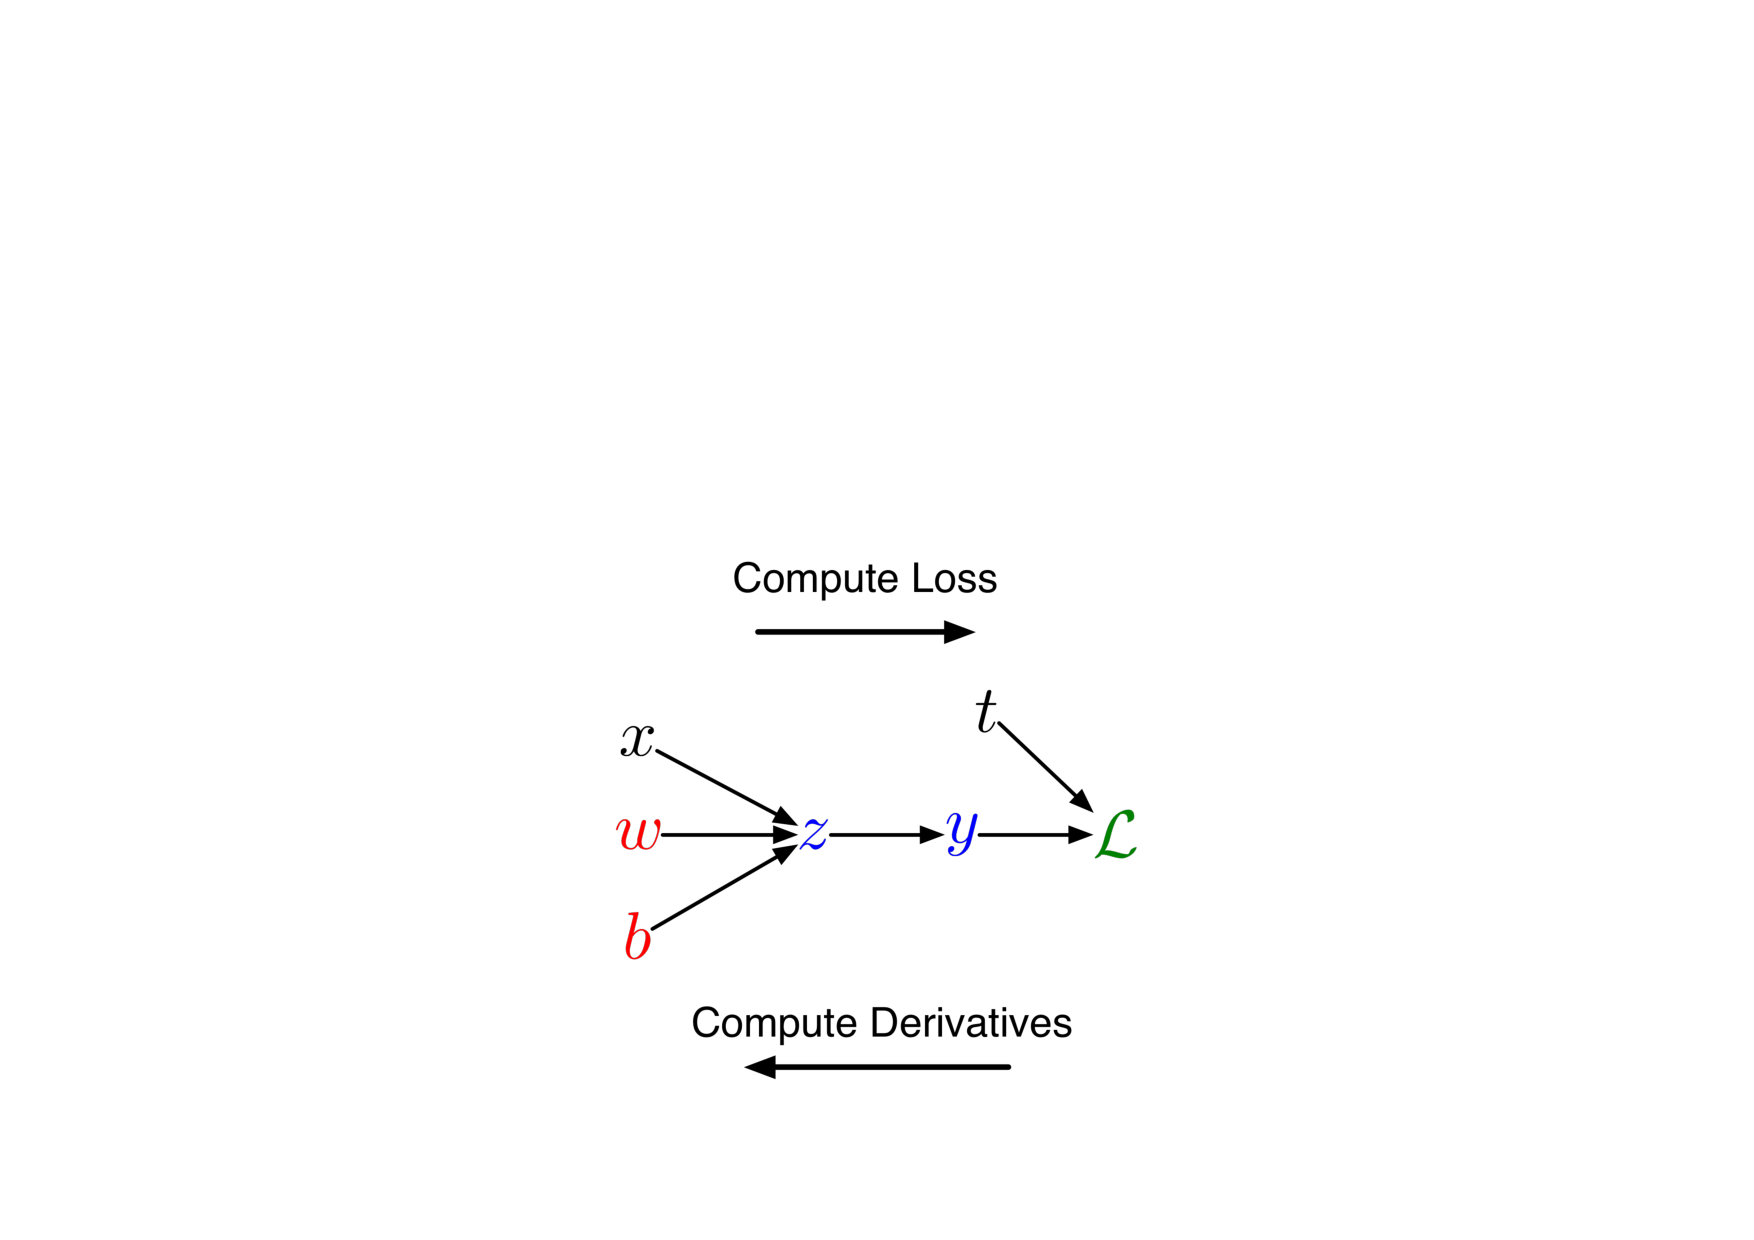
\includegraphics[width=0.5\textwidth]{graphics/comp_graph}
\par\end{center}
\begin{itemize}
\item \textcolor{magenta}{Loss }is computed in the \textcolor{magenta}{forward}
pass
\item \textcolor{magenta}{Gradient} is computed in the \textcolor{magenta}{backward}
pass
\begin{itemize}
\item the derivatives of $y$ and $z$ are \textcolor{magenta}{exact/known}
\item the derivatives of $\mathcal{L}$ are \textcolor{magenta}{computed},
starting from the end
\item the gradients wrt to the parameters are readily obtained by \textcolor{magenta}{backpropagation}
using the\textcolor{magenta}{{} chain rule}!
\end{itemize}
\end{itemize}

\foilhead{Backprop in Practice}
\begin{itemize}
\item Consider the function
\[
f(x,y)=\frac{x+\sigma(y)}{\sigma(x)+(x+y)^{2}},\quad\sigma(x)=\frac{1}{1+e^{-x}}
\]
\item TBC... (exercise)
\end{itemize}

\foilhead{Full Backprop Algorithm}
\begin{center}
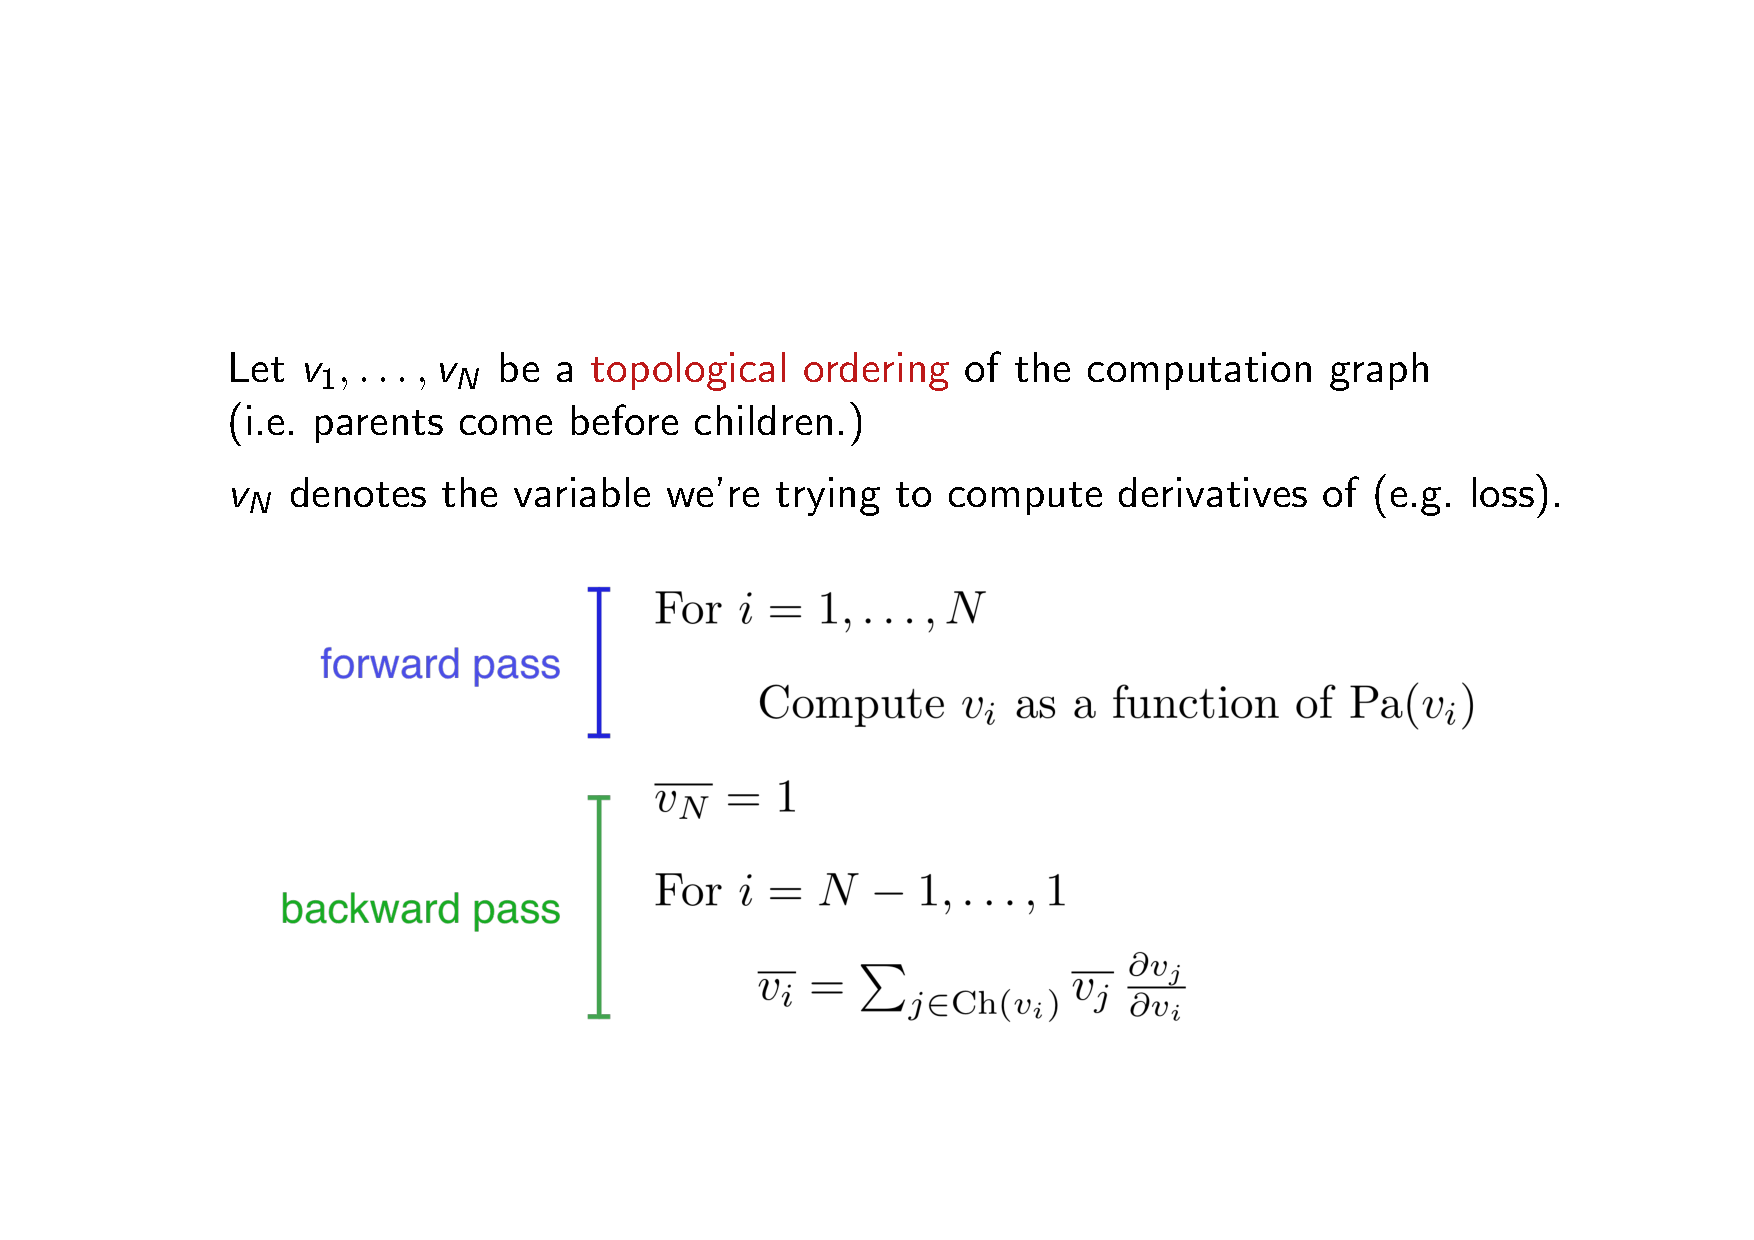
\includegraphics[width=1\textwidth]{graphics/backprop_algo}
\par\end{center}

where $\bar{v}_{i}$ denotes the derivatives of the loss function
with respect to $v_{i},$
\[
\frac{\partial\mathcal{L}}{\partial v_{i}}
\]

\begin{itemize}
\item \textcolor{magenta}{Computational cost} of backprop: approximately
two forward passes, and hence \textcolor{magenta}{linear} in the number
of unknowns
\begin{itemize}
\item Backprop is used to train the overwhelming majority of \textcolor{magenta}{neural
nets} today. 
\item \textcolor{magenta}{Optimization} algorithms, in addition to gradient
descent (e.g. second-order methods) use backprop to compute the gradients.
\item Backprop can thus be used in \textcolor{magenta}{SciML}, and in particular
for Digital Twins (direct and inverse problems), wherever derivatives
and/or gradients need to be computed.
\end{itemize}
\end{itemize}

\foilhead{$\;$}

\vfill{}

\begin{center}
{\Large\textbf{\textcolor{blue}{AUTOGRAD}}}{\Large\par}
\par\end{center}

\vfill{}


\foilhead{Autograd}
\begin{itemize}
\item \texttt{\textcolor{blue}{Autograd}} can automatically differentiate
native Python and Numpy code. 
\begin{itemize}
\item It can handle a \textcolor{magenta}{large subset} of Python's features,
including loops, ifs, recursion and closures.
\item It can even take \textcolor{magenta}{derivatives} of \textcolor{magenta}{derivatives}
of \textcolor{magenta}{derivatives}, etc. 
\item It supports \textcolor{magenta}{reverse-mode differentiation} (a.k.a.
\textcolor{magenta}{backpropagation}), which means it can efficiently
take gradients of scalar-valued functions with respect to array-valued
arguments, as well as \textcolor{magenta}{forward-mode differentiation}
(to compute sensitivities), and the two can be composed arbitrarily. 
\item The main intended application of Autograd is \textcolor{red}{gradient-based
optimization}.
\end{itemize}
\item After a function is evaluated, \texttt{\textcolor{blue}{Autograd}}
has a \textcolor{magenta}{graph} specifying all operations that were
performed on the inputs with respect to which we want to differentiate. 
\begin{itemize}
\item This is the\textcolor{magenta}{{} computational graph} of the function
evaluation. 
\item To compute the derivative, we simply apply the basic rules of (analytical)
differentiation to each \textcolor{magenta}{node} in the graph.
\end{itemize}
\item \textcolor{magenta}{Reverse mode differentiation}
\begin{itemize}
\item Given a function made up of several nested function calls, there are
several ways to compute its derivative.
\item For example, given
\[
L(x)=F(G(H(x))),
\]
 the chain rule says that its gradient is 
\[
\mathrm{d}L/\mathrm{d}x=\mathrm{d}F/\mathrm{d}G*\mathrm{d}G/\mathrm{d}H*\mathrm{d}H/\mathrm{d}x.
\]
\item If we evaluate this product from right-to-left: 
\[
(\mathrm{d}F/\mathrm{d}G*(\mathrm{d}G/\mathrm{d}H*\mathrm{d}H/\mathrm{d}x)),
\]
 the same order as the computations themselves were performed, this
is called \textcolor{magenta}{forward-mode differentiation}. 
\item If we evaluate this product from left-to-right: 
\[
((\mathrm{d}F/\mathrm{d}G*\mathrm{d}G/\mathrm{d}H)*\mathrm{d}H/\mathrm{d}x),
\]
the reverse order as the computations themselves were performed, this
is called \textcolor{magenta}{reverse-mode differentiation}.
\end{itemize}
\item Compared to finite differences or forward-mode, reverse-mode differentiation
is by far the more practical method for differentiating functions
that take in a (very)\textcolor{magenta}{{} large vector }and output
a single number. 
\item In the machine learning community, reverse-mode differentiation is
known as\textcolor{magenta}{{} 'backpropagation',} since the gradients
propagate backwards through the function (as seen above).
\item It's particularly nice since you don't need to instantiate the intermediate
Jacobian matrices explicitly, and instead only rely on applying a
sequence of matrix-free \textcolor{magenta}{vector-Jacobian product
}functions (VJPs). 
\item Because Autograd supports \textcolor{magenta}{higher derivatives}
as well, \textcolor{magenta}{Hessian}-vector products (a form of second-derivative)
are also available and efficient to compute.
\end{itemize}
\begin{rem*}
Autograd is now being superseded by \texttt{\textcolor{blue}{JAX}}.
\end{rem*}

\foilhead{$\;$}

\vfill{}

\begin{center}
{\Large\textbf{\textcolor{blue}{EXAMPLES}}}{\Large\par}
\par\end{center}

\vfill{}


\foilhead{Bibliography}
\begin{thebibliography}{1}
\bibitem{Baydin2018} A. Baydin, B. Pearlmutter, A. Radul, J. Siskind.
Automatic differentitation in machine learning: a survey. \emph{Journal
of Machine Learning Research,} 18 (2017), article 153.

\bibitem{Asch2022}M. Asch. \emph{Digital Twins: from Model-Based
to Data-Driven.} SIAM, 2022.

\bibitem{Asch2016}M. Asch, M. Bocquet, M. Nodet. \emph{Data Assimilation:
Theory, Algorithms and Applications.} SIAM, 2016.

\end{thebibliography}

\end{document}
